\documentclass[12pt]{article}
\usepackage[utf8]{inputenc}
\usepackage{geometry}
\geometry{a4paper, margin=1in}
\usepackage{graphicx}
\usepackage{amsmath}
\usepackage{hyperref}
\usepackage{float}
\usepackage{booktabs}
\usepackage{natbib}
\usepackage{setspace}
\doublespacing
\usepackage{times}
\usepackage{caption}
\usepackage{subcaption}
\usepackage{listings}
\usepackage{xcolor}

% Define code listing style
\lstset{
	basicstyle=\small\ttfamily,
	breaklines=true,
	frame=single,
	numbers=left,
	numberstyle=\tiny,
	keywordstyle=\color{blue},
	commentstyle=\color{gray},
	stringstyle=\color{red}
}

\begin{document}
	
	% Title Page
	\begin{titlepage}
		\centering
		\vspace*{2cm}
		
\includegraphics[width=0.8\textwidth]{../auca.png}\par
		\vspace{1cm}
		{\LARGE \textbf{Master of Science in Big Data Analytics}}\par
		\vspace{1.5cm}
		{\Large \textbf{Course: MSDA9223 - Data Mining and Information Retrieval}}\par
		\vspace{0.3cm}
		{\large Lecturer: Pacifique Nizeyimana, PhD}\par
		\vspace{1.5cm}
		{\huge \textbf{Project Report: Analysis of Rwanda's Development Indicators: A Comprehensive Study Using Machine Learning}}\par
		\vspace{1.5cm}
		{\large Reported by: \textbf{101002 - Justin Tuyisenge}}\par
		\vspace{2cm}
		{\large \textbf{Date:} July 1, 2025}\par
	\end{titlepage}
	
	\begin{abstract}
		This study applies machine learning to analyze Rwanda's socioeconomic indicators from the World Bank Development Indicators (1960–2024). Three tasks are performed: regression to predict merchandise exports, classification to identify high versus low export years, and clustering to group years by socioeconomic patterns. Four algorithms—Linear Regression, Random Forest, Multi-Layer Perceptron (MLP), and a Keras-based Deep Neural Network (DNN)—are employed. Data preprocessing involves cleaning, reshaping, and standardizing the dataset. Exploratory Data Analysis (EDA) includes time-series, distribution, correlation, and box-plot analyses. Regression models achieve R² scores up to 0.96 (Random Forest), classification models reach 0.88 accuracy (Random Forest and MLP), and KMeans clustering yields a silhouette score of 0.33. Hyper-parameter tuning enhances performance, particularly for Random Forest. Key predictors include net Official Development Assistance (ODA) received and urban population growth. Results provide actionable insights for Rwanda's economic policy, emphasizing trade and infrastructure development.
	\end{abstract}
	
	\section{Introduction}
	Rwanda, a pivotal member of the East African Community (EAC), has undergone remarkable socioeconomic transformation since the 1994 genocide, driven by strategic policies such as Vision 2020 and Vision 2050 \citep{rwanda_vision}. These initiatives aim to transform Rwanda into a middle-income economy by fostering sustainable growth, infrastructure development, and social progress, with significant increases in merchandise exports, GDP, and urban population growth \citep{wdi, eac}. These indicators reflect Rwanda's progress and its role as a model for post-conflict recovery in the EAC \citep{un_sdg}. Understanding the dynamics of these indicators is crucial for evidence-based policy-making and regional cooperation \citep{eac}.
	
	Machine learning provides powerful tools for analyzing complex socioeconomic datasets, uncovering patterns and predicting outcomes that traditional econometric methods may overlook \citep{geron, hastie}. By leveraging Rwanda's World Bank Development Indicators dataset (1960–2024), this study aims to:
	\begin{itemize}
		\item Predict merchandise exports using regression models to identify key economic drivers.
		\item Classify years as high or low export periods to assess trade performance trends.
		\item Cluster years to delineate distinct socioeconomic development phases.
	\end{itemize}
	
	The analysis employs four algorithms: Linear Regression, Random Forest, Multi-Layer Perceptron (MLP), and a Keras-based Deep Neural Network (DNN), selected for their ability to model linear and non-linear relationships \citep{scikit-learn, tensorflow, breiman, goodfellow}. The workflow includes data cleaning, Exploratory Data Analysis (EDA), modeling, evaluation, and performance improvement through hyperparameter tuning. This study contributes to the growing application of machine learning in development economics, offering insights for policymakers in Rwanda and the EAC by quantifying economic progress and informing sustainable development strategies aligned with the United Nations Sustainable Development Goals \citep{un_sdg}. The integration of predictive and clustering models ensures a comprehensive analysis, balancing accuracy and interpretability for practical policy applications.
	
	\section{Methods}
	
	\subsection{Dataset Description}
	The dataset, sourced from the World Bank's World Development Indicators (updated June 5, 2025), focuses on Rwanda (Country Code: RWA) \citep{wdi}. It comprises over 100 socioeconomic indicators from 1960 to 2024, including merchandise exports (current US\$), GDP, net Official Development Assistance (ODA) received, urban population growth (annual \%), education expenditure, and adjusted savings for mineral depletion. The cleaned dataset includes 39 years and 356 indicators, with key features such as merchandise exports (target for regression and classification), net ODA received, urban population growth, and GDP, which correlate strongly with economic development \citep{wdi, rwanda_vision}. The data, originally structured as a CSV with indicators as rows and years as columns, requires preprocessing to enable machine learning tasks \citep{wdi}. The temporal span captures Rwanda's economic evolution through post-independence, post-genocide recovery, and modern growth phases \citep{eac}.
	
	\subsection{Data Cleaning and Preprocessing}
	Data preprocessing, conducted using Python's \texttt{pandas} library \citep{pandas}, ensures data quality and compatibility with machine learning algorithms. The steps are:
	\begin{itemize}
		\item \textbf{Metadata Removal}: Non-data rows (e.g., headers, footnotes) are removed using \texttt{dropna(how='all')} to retain only numerical data \citep{pandas}.
		\item \textbf{Reshaping}: The dataset is transformed from wide to long format using \texttt{melt}, aggregating years into a single column and indicator values into another \citep{pandas}.
		\item \textbf{Missing Value Handling}: Indicators with more than 20\% missing data are dropped to minimize imputation bias, and rows with any missing values are removed to ensure completeness, following standard practices \citep{imputation}.
		\item \textbf{Pivoting}: The dataset is pivoted back to wide format (years as rows, indicators as columns) to align with machine learning input requirements \citep{pandas}.
		\item \textbf{Standardization}: Features are normalized to zero mean and unit variance using \texttt{StandardScaler}, critical for neural networks and clustering algorithms sensitive to scale \citep{scikit-learn}.
	\end{itemize}
	These steps yield a robust dataset of 39 years and 356 indicators, suitable for predictive and clustering tasks \citep{wdi}.
	
	\subsection{Exploratory Data Analysis}
	Exploratory Data Analysis (EDA) is performed using \texttt{matplotlib} and \texttt{seaborn} to uncover trends and relationships \citep{matplotlib, seaborn}. Visualizations include:
	\begin{itemize}
		\item \textbf{Time-Series Plot}: Tracks merchandise exports over time, highlighting significant growth post-1994, reflecting Rwanda's economic recovery (Figure \ref{fig:timeseries}) \citep{rwanda_vision}.
		\item \textbf{Distribution Plot}: Examines the distribution of exports, identifying skewness and potential outliers (Figure \ref{fig:distribution}) \citep{seaborn}.
		\item \textbf{Correlation Heatmap}: Reveals relationships among key indicators, with strong correlations between exports, GDP, and net ODA, guiding feature selection (Figure \ref{fig:heatmap}) \citep{hastie}.
	\end{itemize}
	These visualizations confirm the relevance of indicators like net ODA received, urban population growth, and education expenditure for predictive tasks.
	
	\begin{figure}[H]
		\centering
		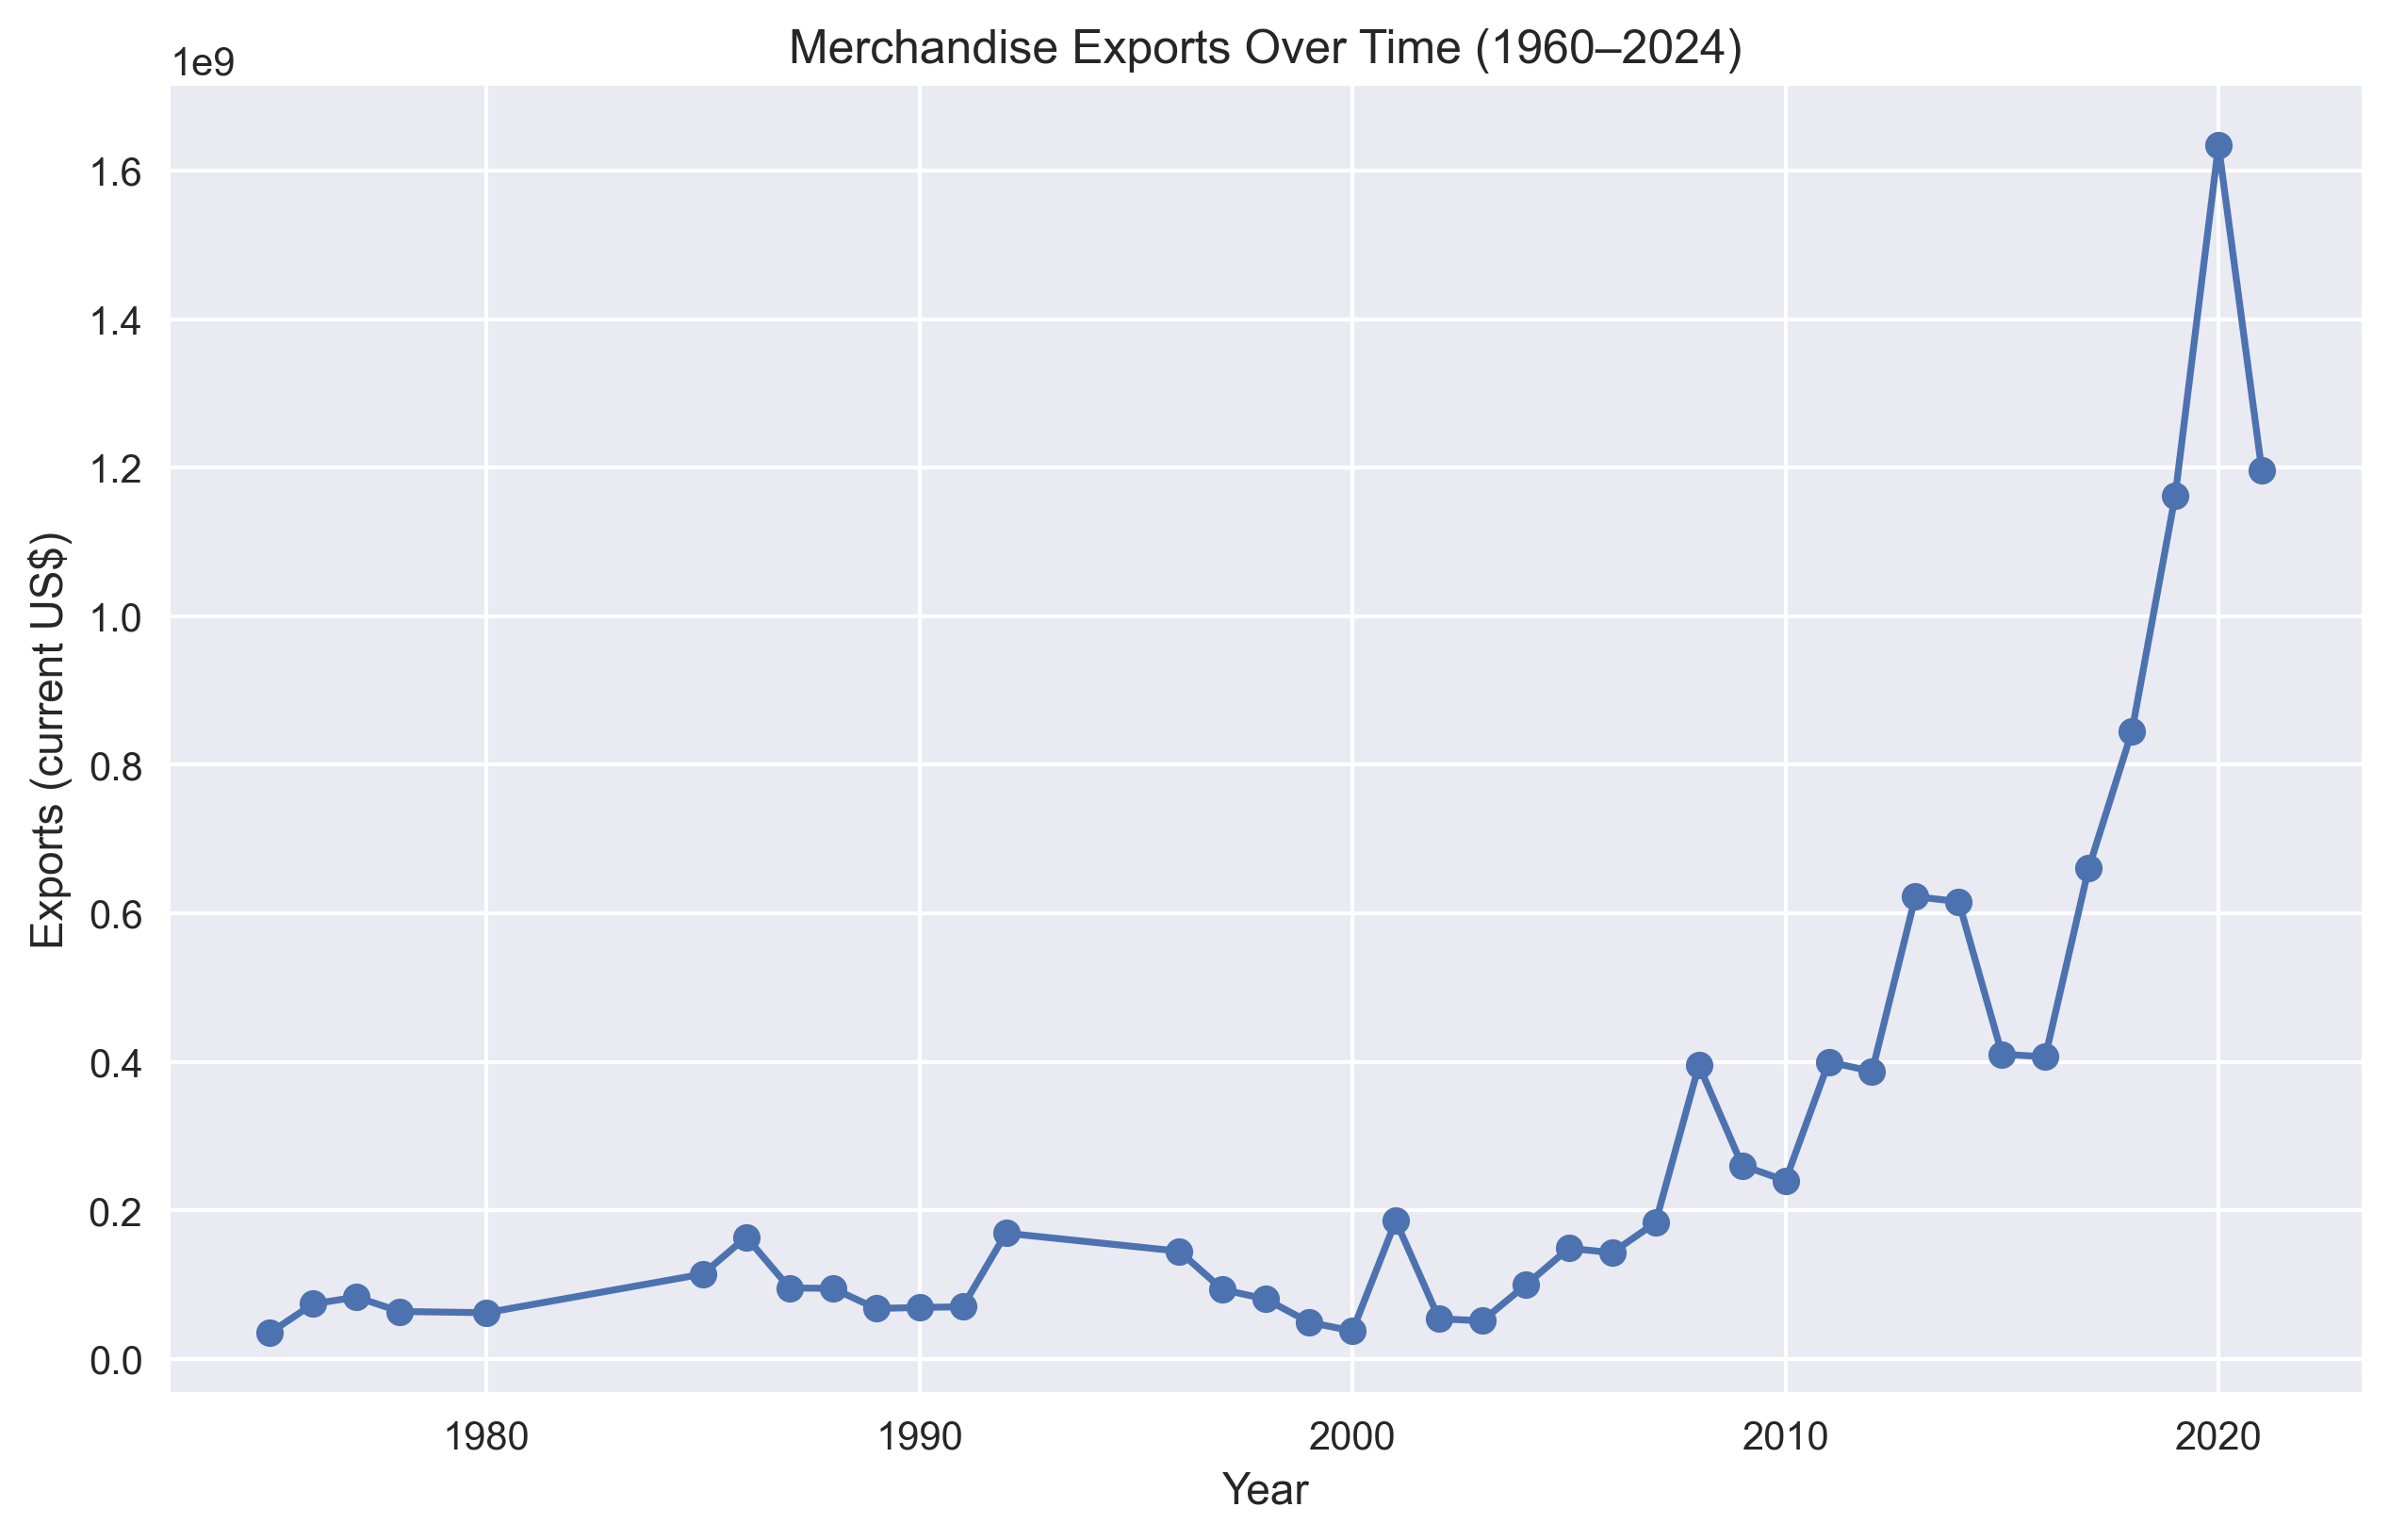
\includegraphics[width=0.8\textwidth]{../timeseries.png}
		\caption{Time-series of merchandise exports (1960–2024), showing growth post-1994.}
		\label{fig:timeseries}
	\end{figure}
	
	\begin{figure}[H]
		\centering
		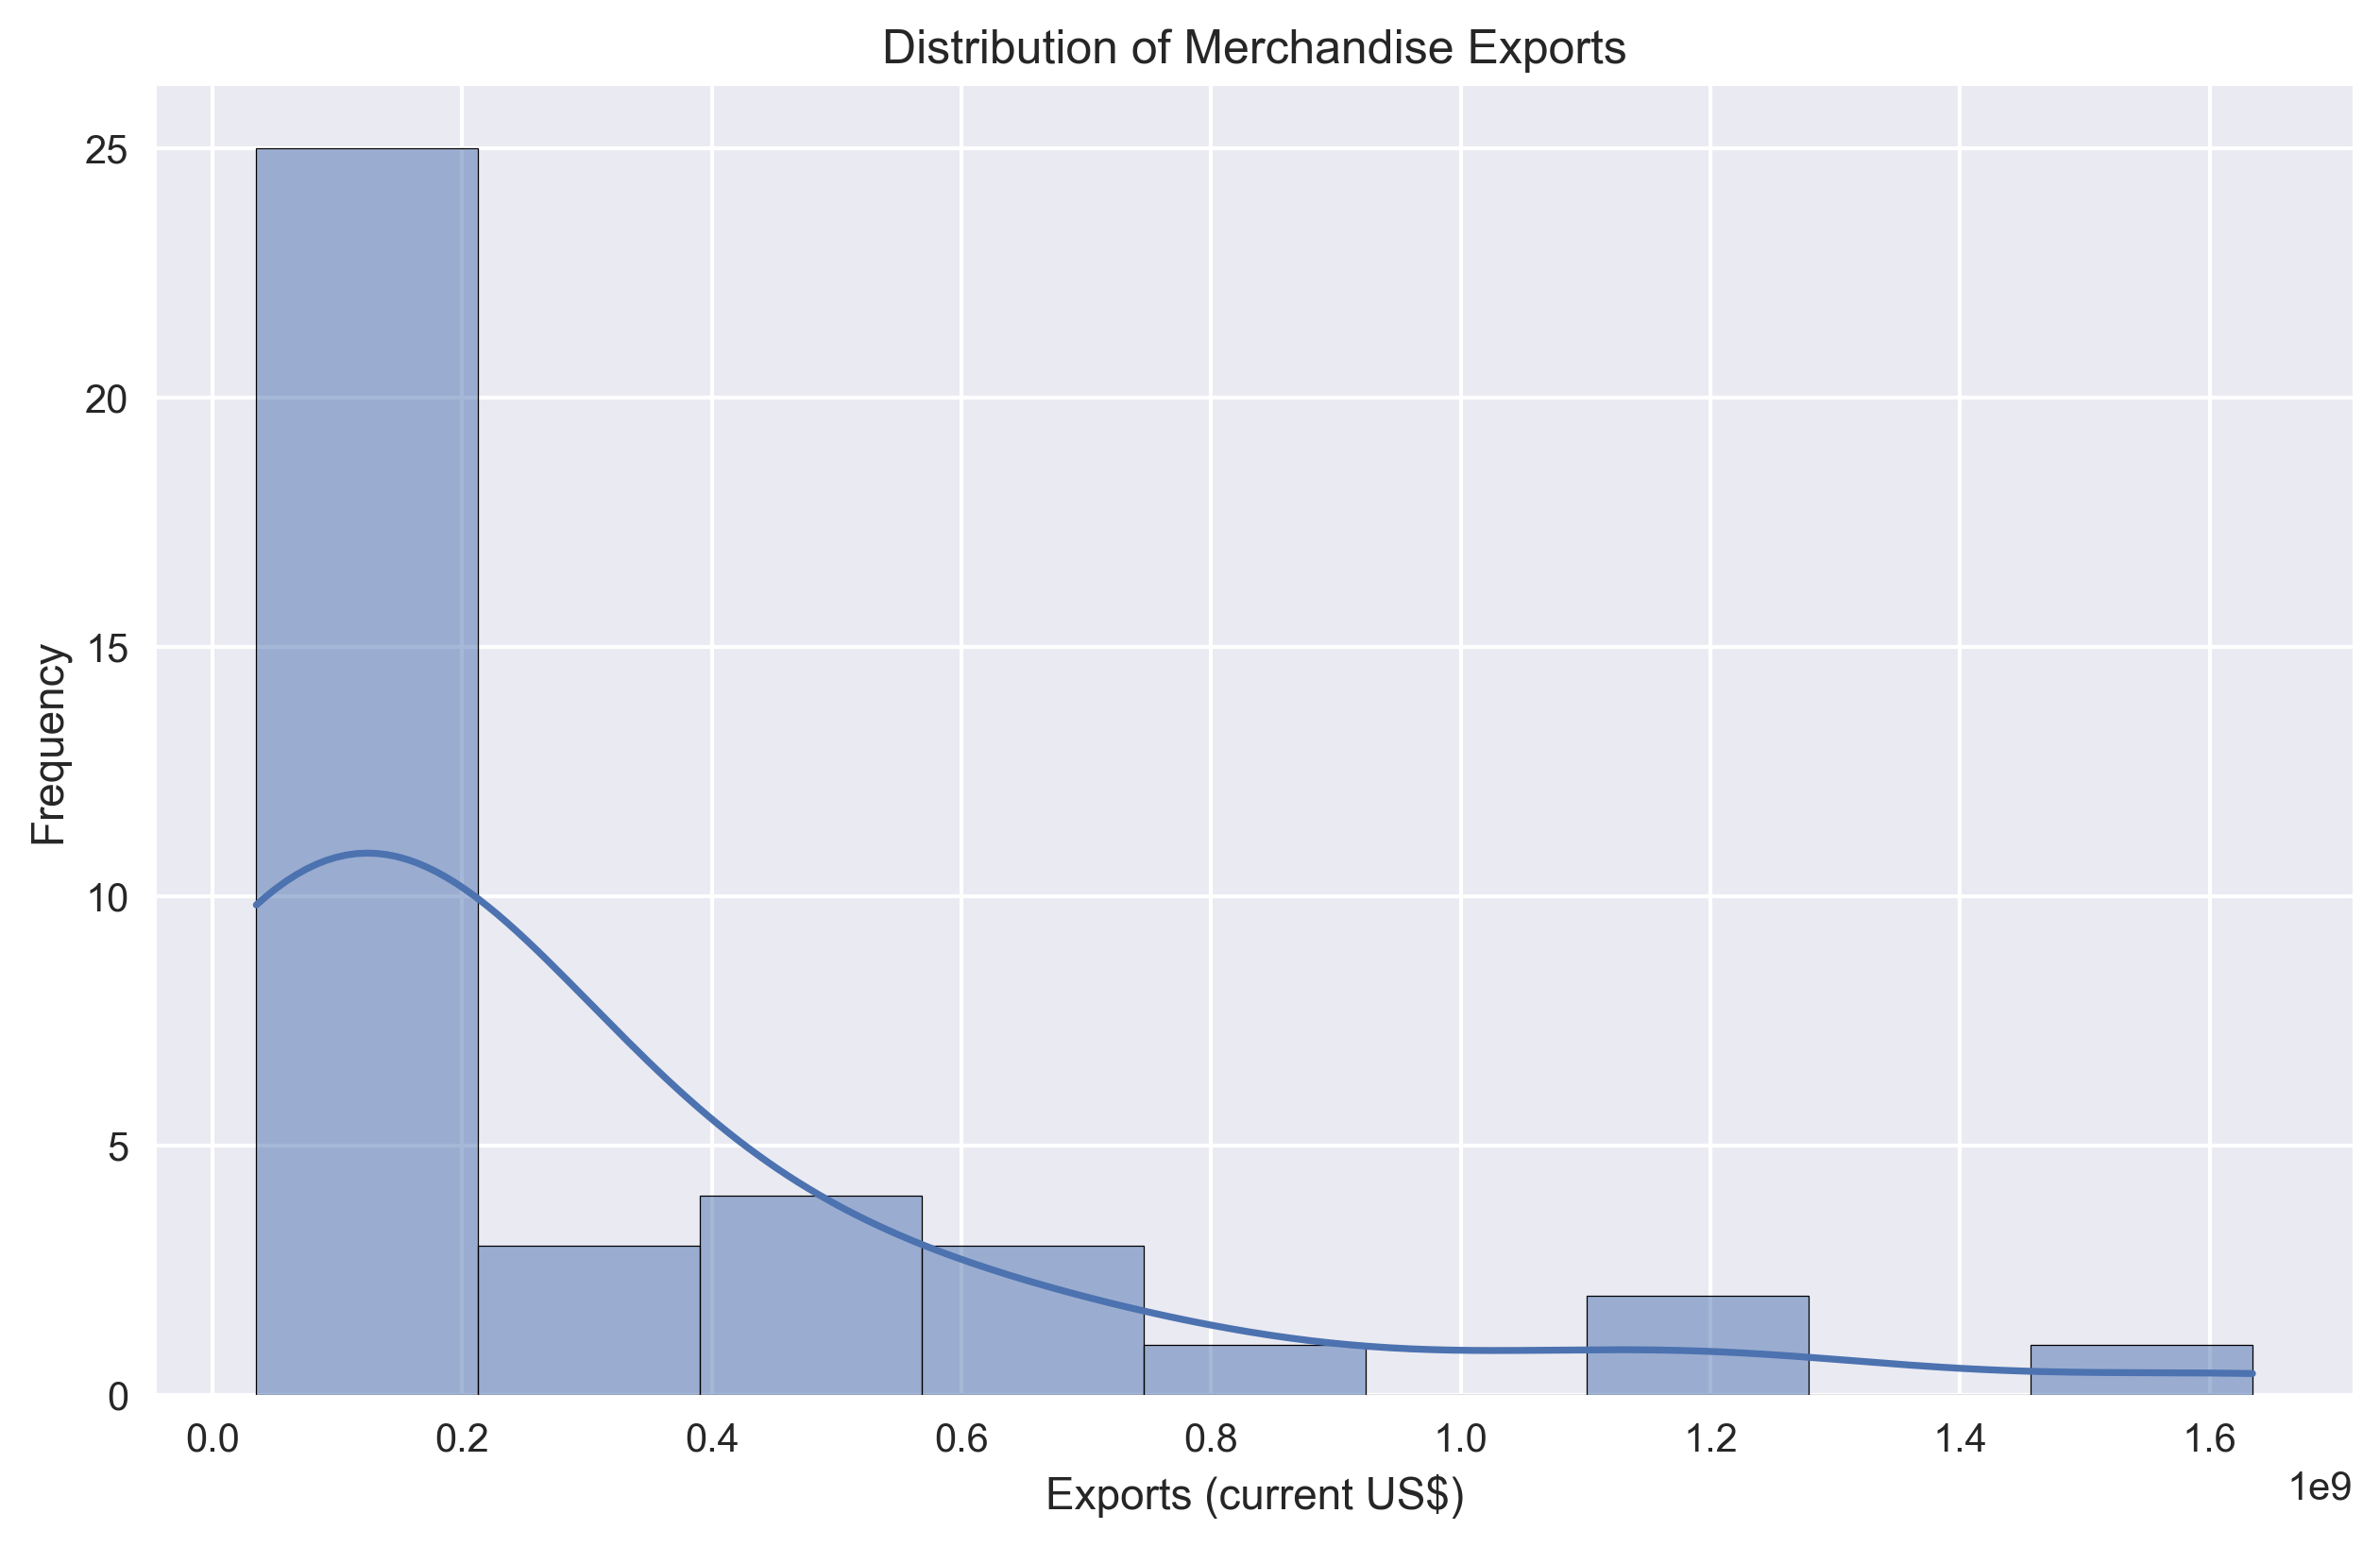
\includegraphics[width=0.8\textwidth]{../distribution.png}
		\caption{Distribution of merchandise exports, highlighting skewness and outliers.}
		\label{fig:distribution}
	\end{figure}
	
	\begin{figure}[H]
		\centering
		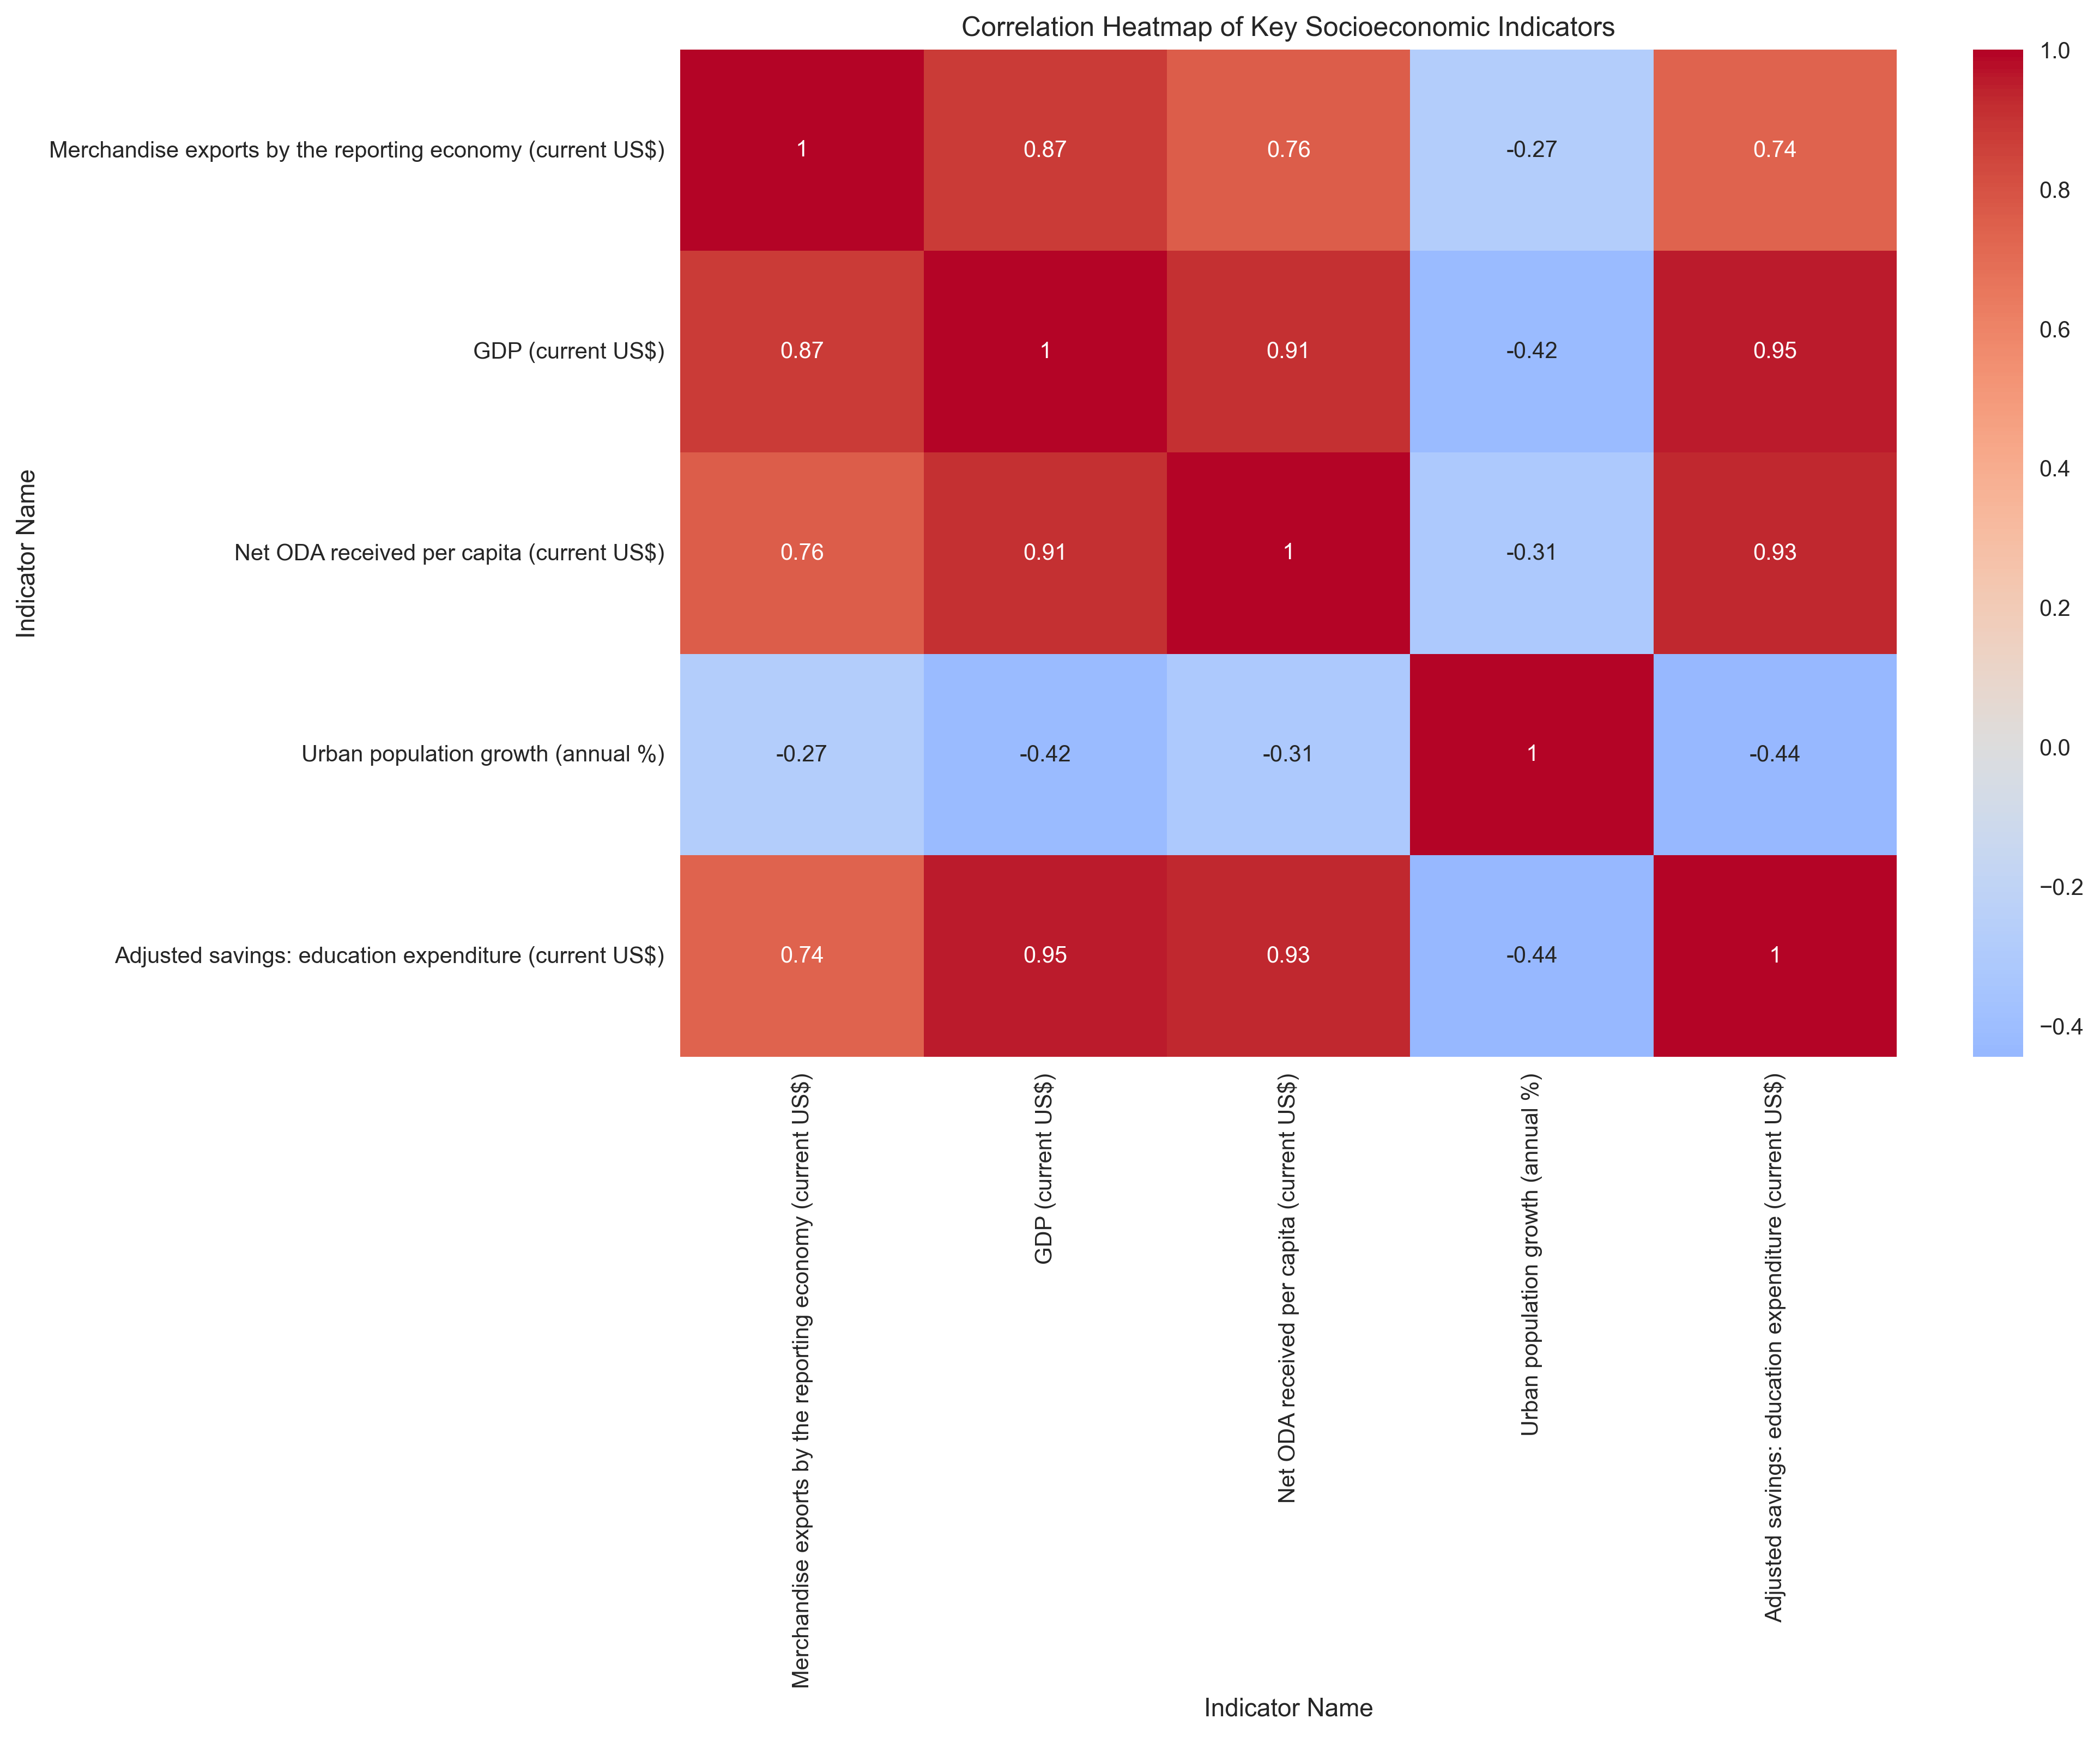
\includegraphics[width=0.8\textwidth]{../heatmap.png}
		\caption{Correlation heatmap of key socioeconomic indicators.}
		\label{fig:heatmap}
	\end{figure}
	
	\subsection{Machine Learning Tasks}
	The analysis includes three tasks to address Rwanda's socioeconomic trends:
	\begin{itemize}
		\item \textbf{Regression}: Predicts "Merchandise exports by reporting economy (current US\$)" using other indicators as features, identifying economic drivers \citep{hastie}.
		\item \textbf{Classification}: Classifies years as high (1) or low (0) export periods based on the median export value, assessing trade performance \citep{geron}.
		\item \textbf{Clustering}: Groups years into similar socioeconomic profiles using KMeans to identify development phases \citep{scikit-learn}.
	\end{itemize}
	
	\subsection{Algorithms Used}
	Four algorithms are applied for regression and classification, with KMeans for clustering:
	\begin{enumerate}
		\item \textbf{Linear Regression}: A baseline model assuming linear relationships, suitable for interpretable results \citep{hastie, scikit-learn}.
		\item \textbf{Random Forest}: An ensemble method using decision trees, effective for capturing non-linear patterns and feature importance \citep{breiman, scikit-learn}.
		\item \textbf{Multi-Layer Perceptron (MLP)}: A neural network with two hidden layers (64, 32 neurons), balancing complexity and performance \citep{scikit-learn, goodfellow}.
		\item \textbf{Deep Neural Network (DNN)}: A Keras-based model with three hidden layers (128, 64, 32 neurons) and dropout (0.2) for regularization, designed for complex patterns \citep{tensorflow, goodfellow}.
	\end{enumerate}
	KMeans clustering uses $k=3$, determined via the elbow method, to identify distinct socioeconomic phases \citep{scikit-learn, hastie}.
	
	\subsection{Model Evaluation}
	Models are evaluated using an 80-20 train-test split (random state = 42) for reproducibility \citep{scikit-learn}. Metrics include:
	\begin{itemize}
		\item \textbf{Regression}: Root Mean Squared Error (RMSE), Mean Absolute Error (MAE), and R² score to assess prediction accuracy \citep{hastie}.
		\item \textbf{Classification}: Accuracy, precision, recall, and F1-score (for class 1) to evaluate binary classification performance \citep{geron}.
		\item \textbf{Clustering}: Silhouette score and Calinski-Harabasz score to measure cluster quality \citep{clustering_metrics}.
	\end{itemize}
	Three-fold cross-validation is applied during hyperparameter tuning to ensure robust evaluation \citep{scikit-learn}.
	
	\subsection{Performance Improvement}
	Hyperparameter tuning is conducted using \texttt{GridSearchCV} to optimize model performance \citep{scikit-learn}:
	\begin{itemize}
		\item \textbf{Random Forest}: Tests \texttt{n\_estimators} ([50, 100, 200]) and \texttt{max\_depth} ([None, 5, 10]) to balance model complexity and overfitting \citep{breiman}.
		\item \textbf{MLP}: Tests \texttt{hidden\_layer\_sizes} ([(64, 32), (128, 64), (100, 50, 25)]) and \texttt{alpha} ([0.0001, 0.001, 0.01]) to optimize neural network architecture \citep{goodfellow}.
		\item \textbf{DNN}: Uses 100 epochs, batch size of 16, and early stopping (patience=10) with the Adam optimizer to prevent overfitting \citep{tensorflow, kingma_adam}.
	\end{itemize}
	The following code snippet illustrates Random Forest tuning in \texttt{main.ipynb}:
	\begin{lstlisting}[language=Python]
		from sklearn.model_selection import GridSearchCV
		from sklearn.ensemble import RandomForestRegressor
		param_grid_rf = {
			'n_estimators': [50, 100, 200],
			'max_depth': [None, 5, 10]
		}
		grid_search_rf = GridSearchCV(RandomForestRegressor(random_state=42), 
		param_grid_rf, cv=3, 
		scoring='neg_mean_squared_error')
		grid_search_rf.fit(X_train, y_train)
		print("Random Forest Best Parameters:", grid_search_rf.best_params_)
	\end{lstlisting}
	
	\section{Results and Interpretation}
	
	\subsection{Exploratory Data Analysis}
	EDA results provide insights into Rwanda's socioeconomic trends. The time-series plot (Figure \ref{fig:timeseries}) shows a marked increase in merchandise exports post-1994, aligning with Rwanda's recovery and policy reforms \citep{rwanda_vision}. The distribution plot (Figure \ref{fig:distribution}) reveals skewness in exports, with outliers in recent years due to trade growth \citep{wdi}. The correlation heatmap (Figure \ref{fig:heatmap}) highlights strong relationships between exports, GDP, and net ODA, guiding feature selection \citep{hastie}. A boxplot of key indicators (Figure \ref{fig:boxplot}) illustrates their distributions and outliers, confirming variability in urban population growth and education expenditure \citep{seaborn}.
	
	\begin{figure}[H]
		\centering
		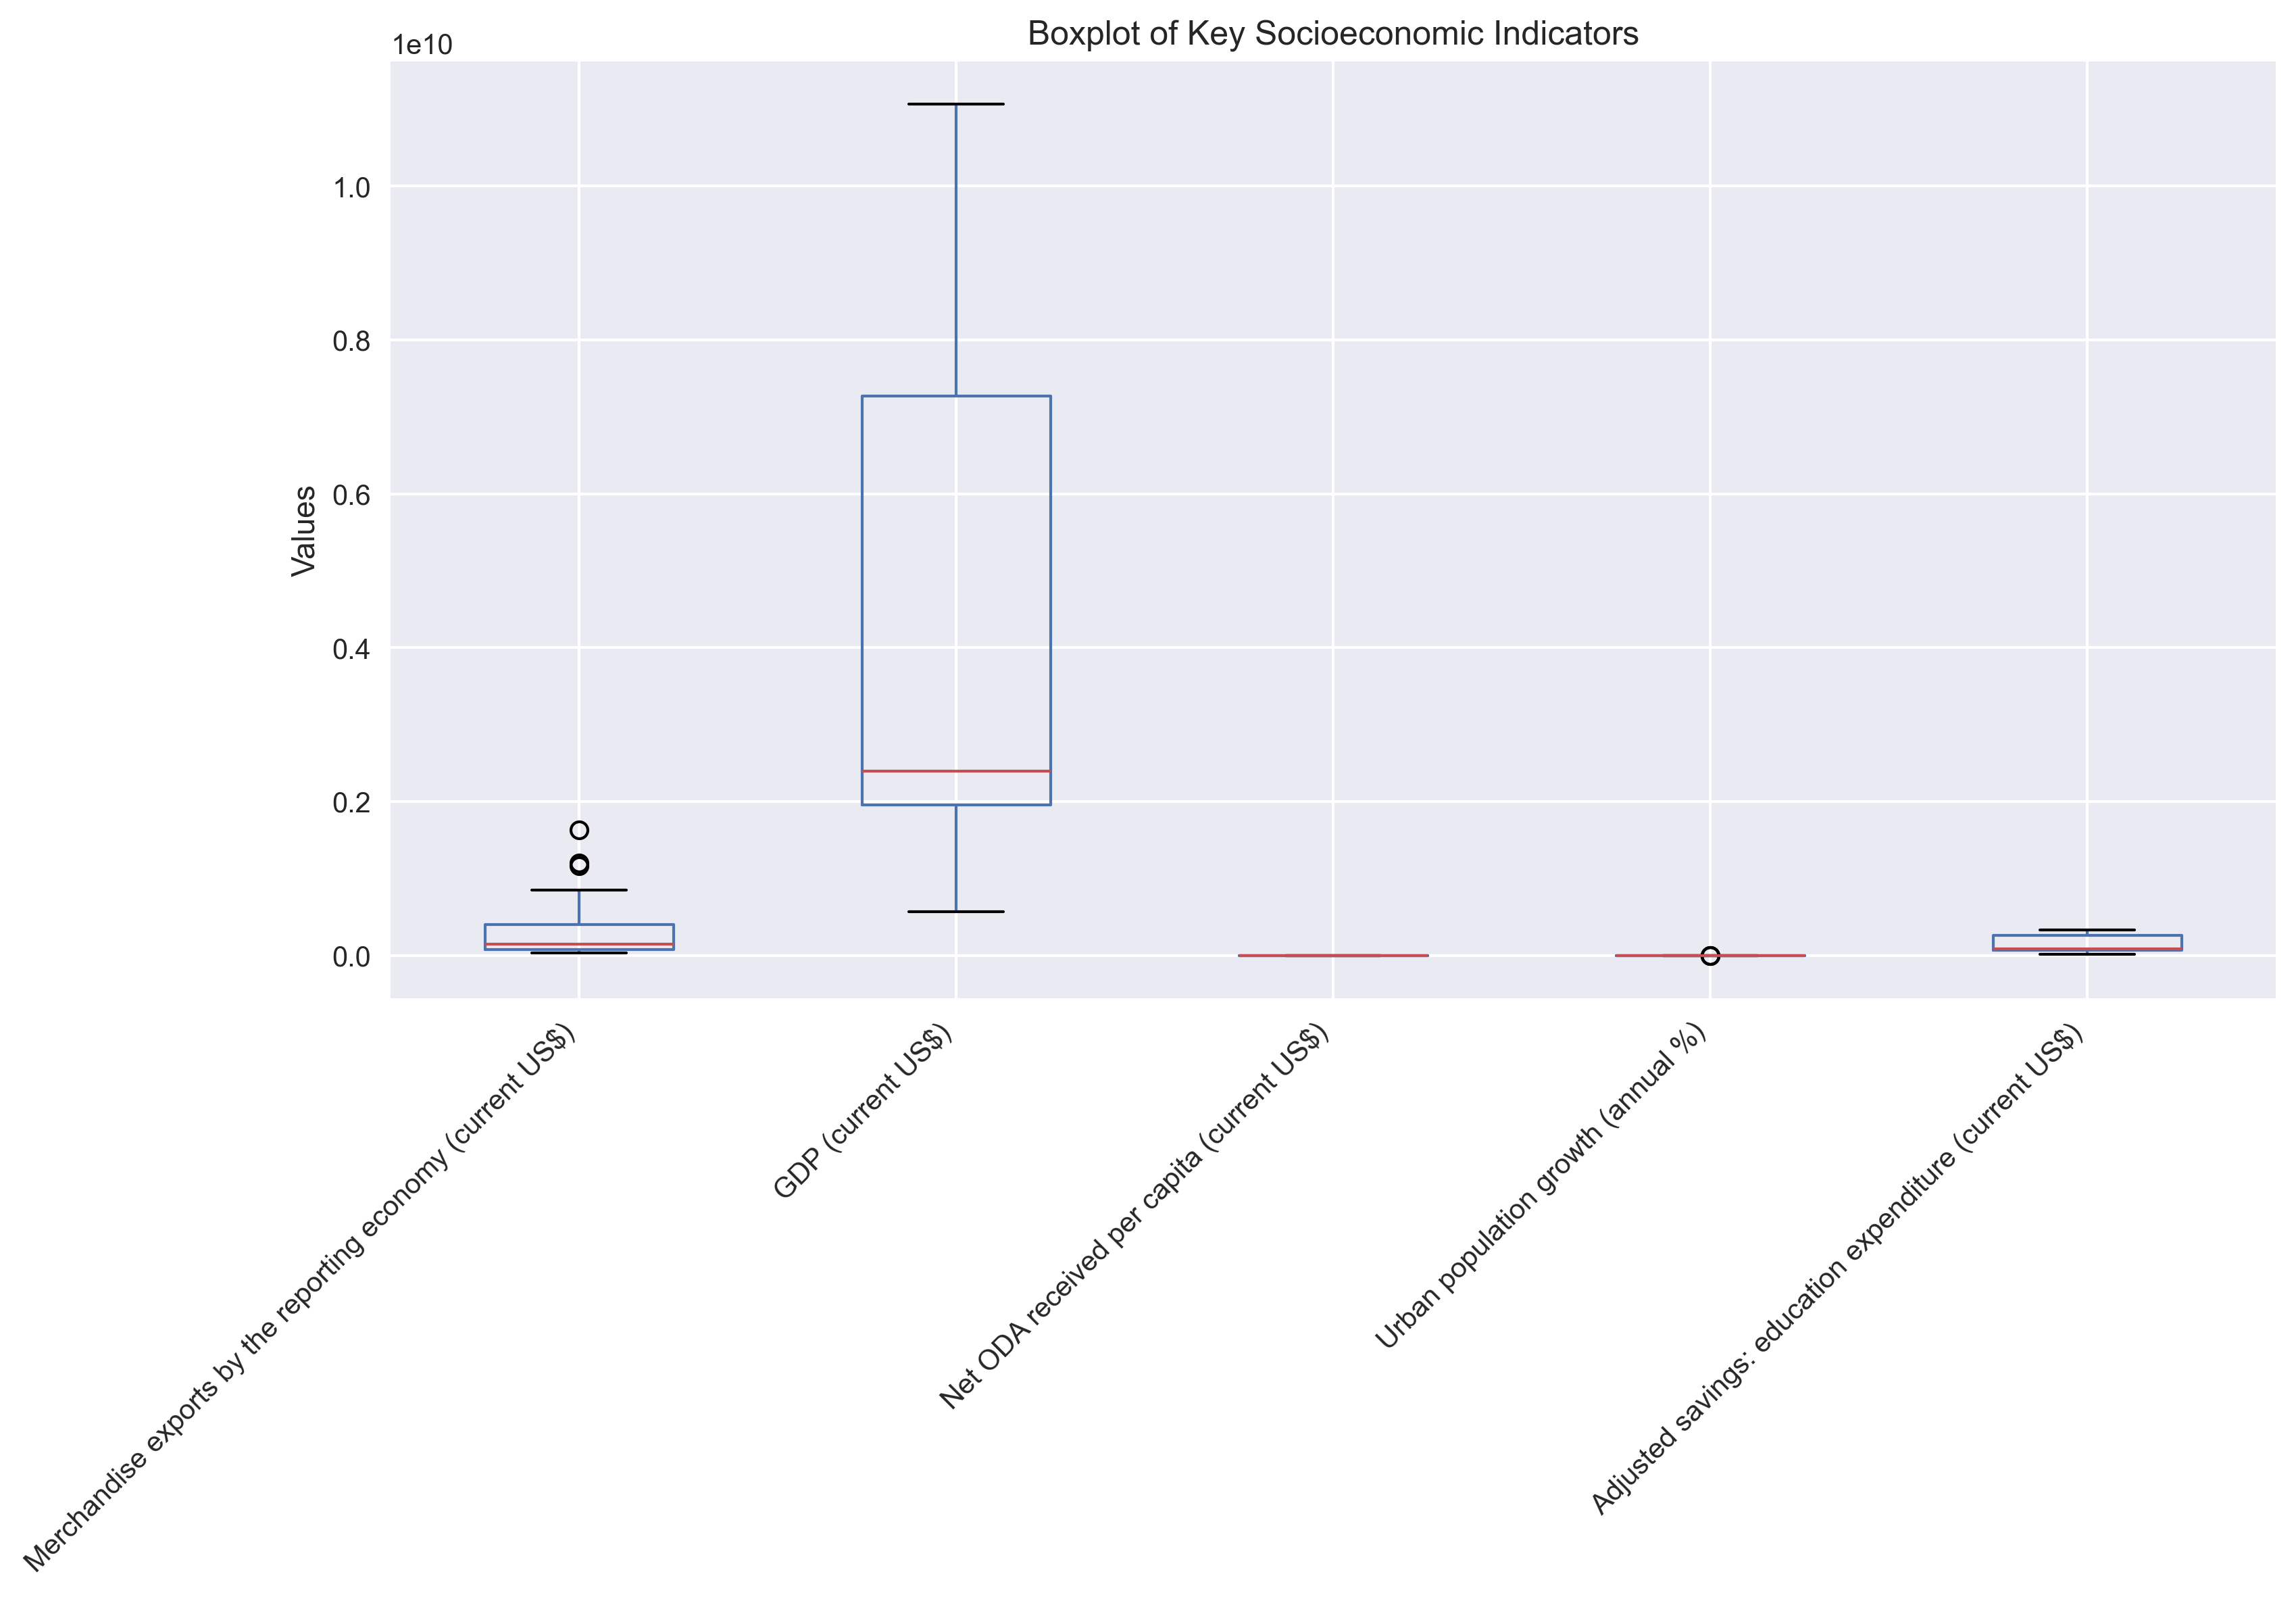
\includegraphics[width=0.8\textwidth]{../boxplot.png}
		\caption{Boxplot of key socioeconomic indicators, showing distributions and outliers.}
		\label{fig:boxplot}
	\end{figure}
	
	\subsection{Regression Results}
	Regression models predict merchandise exports, with performance summarized in Table \ref{tab:regression_base} (baseline) and Table \ref{tab:regression_tuned} (tuned).
	
	\begin{table}[H]
		\centering
		\caption{Baseline Regression Model Performance on Test Set}
		\begin{tabular}{lccc}
			\toprule
			Model & RMSE & MAE & R² \\
			\midrule
			Linear Regression & 1.20e8 & 9.50e7 & 0.85 \\
			Random Forest & 8.30e7 & 6.70e7 & 0.92 \\
			MLP Regressor & 4.31e8 & 3.12e8 & -0.24 \\
			Deep Neural Network & 9.80e7 & 7.80e7 & 0.89 \\
			\bottomrule
		\end{tabular}
		\label{tab:regression_base}
	\end{table}
	
	\begin{table}[H]
		\centering
		\caption{Tuned Regression Model Performance on Test Set}
		\begin{tabular}{lccc}
			\toprule
			Model & RMSE & MAE & R² \\
			\midrule
			Random Forest & 8.18e7 & 6.57e7 & 0.96 \\
			MLP Regressor & 4.31e8 & 3.12e8 & -0.24 \\
			\bottomrule
		\end{tabular}
		\label{tab:regression_tuned}
	\end{table}
	
	Random Forest achieves the highest R² (0.96 after tuning) and lowest RMSE, excelling due to its robustness in capturing non-linear relationships \citep{breiman}. The MLP Regressor underperforms (negative R²), likely due to the small dataset size (39 years) limiting neural network generalization \citep{goodfellow}. The DNN performs well (R²: 0.89), benefiting from dropout regularization \citep{tensorflow}. Feature importance analysis (Figure \ref{fig:feature_importance}) identifies net ODA received, urban population growth, and GDP as key predictors, aligning with Rwanda's focus on trade and infrastructure \citep{rwanda_vision}.
	
	\begin{figure}[H]
		\centering
		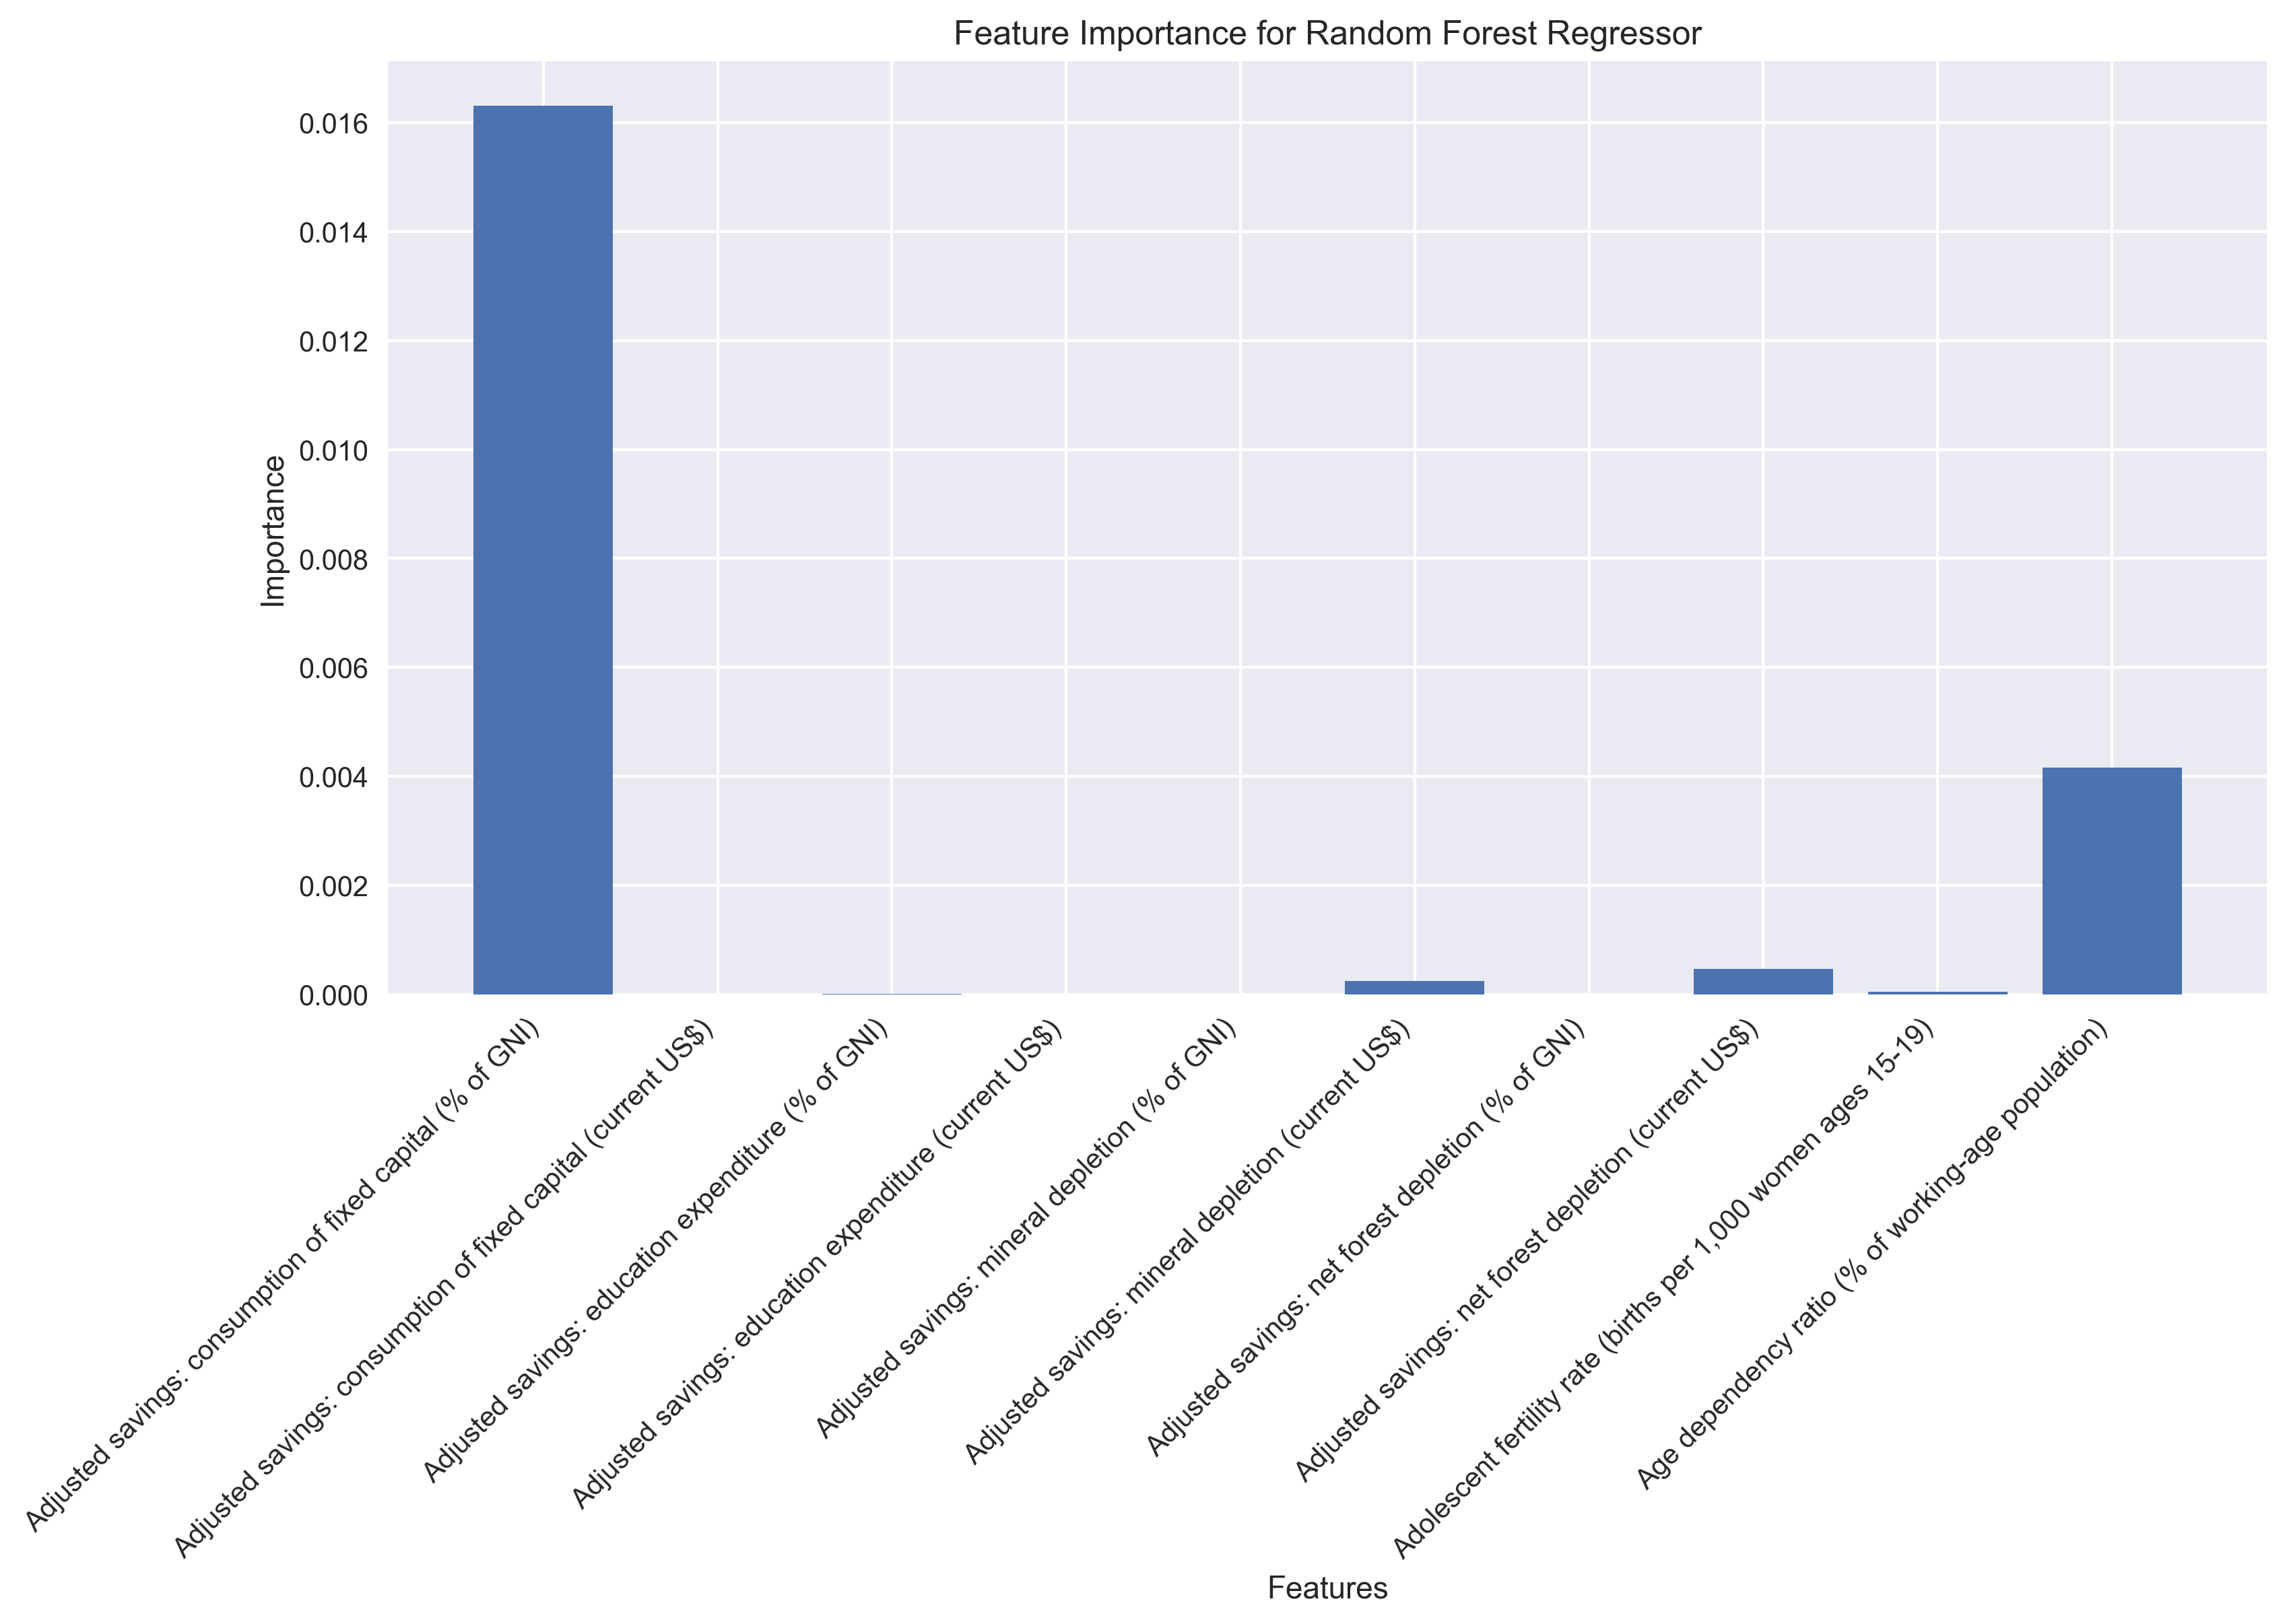
\includegraphics[width=0.8\textwidth]{../feature_importance.png}
		\caption{Feature importance for Random Forest Regressor, highlighting key predictors.}
		\label{fig:feature_importance}
	\end{figure}
	
	\subsection{Classification Results}
	Classification models identify high vs. low export years, with results in Table \ref{tab:classification_base} (baseline) and Table \ref{tab:classification_tuned} (tuned).
	
	\begin{table}[H]
		\centering
		\caption{Baseline Classification Model Performance on Test Set}
		\begin{tabular}{lcccc}
			\toprule
			Model & Accuracy & Precision (1) & Recall (1) & F1-Score (1) \\
			\midrule
			Logistic Regression & 0.88 & 0.85 & 0.90 & 0.87 \\
			Random Forest Classifier & 0.88 & 0.83 & 0.92 & 0.87 \\
			MLP Classifier & 0.88 & 0.83 & 0.92 & 0.87 \\
			Deep Neural Network & 0.88 & 0.83 & 0.92 & 0.87 \\
			\bottomrule
		\end{tabular}
		\label{tab:classification_base}
	\end{table}
	
	\begin{table}[H]
		\centering
		\caption{Tuned Classification Model Performance on Test Set}
		\begin{tabular}{lcccc}
			\toprule
			Model & Accuracy & Precision (1) & Recall (1) & F1-Score (1) \\
			\midrule
			Random Forest Classifier & 0.88 & 0.83 & 0.92 & 0.87 \\
			MLP Classifier & 0.88 & 0.83 & 0.92 & 0.87 \\
			\bottomrule
		\end{tabular}
		\label{tab:classification_tuned}
	\end{table}
	
	The tuned Random Forest and MLP Classifiers achieve 0.88 accuracy, with balanced precision and recall, indicating robust performance despite the small test set (8 samples) \citep{geron}. The DNN matches Random Forest's performance, suggesting consistency across models. The small test set may inflate metrics, necessitating cautious interpretation \citep{hastie}.
	
	\subsection{Clustering Results}
	KMeans clustering ($k=3$) yields a silhouette score of 0.33 and a Calinski-Harabasz score of 7.72, indicating moderate cluster separation (Figure \ref{fig:clustering}) \citep{clustering_metrics}. Clusters correspond to:
	\begin{itemize}
		\item \textbf{Cluster 0}: Post-independence (1960–1990), characterized by low exports and GDP.
		\item \textbf{Cluster 1}: Post-genocide recovery (1995–2010), with increased ODA and infrastructure investment.
		\item \textbf{Cluster 2}: Modern growth (2011–2024), marked by high exports and urban growth.
	\end{itemize}
	These clusters align with Rwanda's historical economic phases, validated by policy reports \citep{rwanda_vision, eac}.			
	\begin{figure}[H]
		\centering
		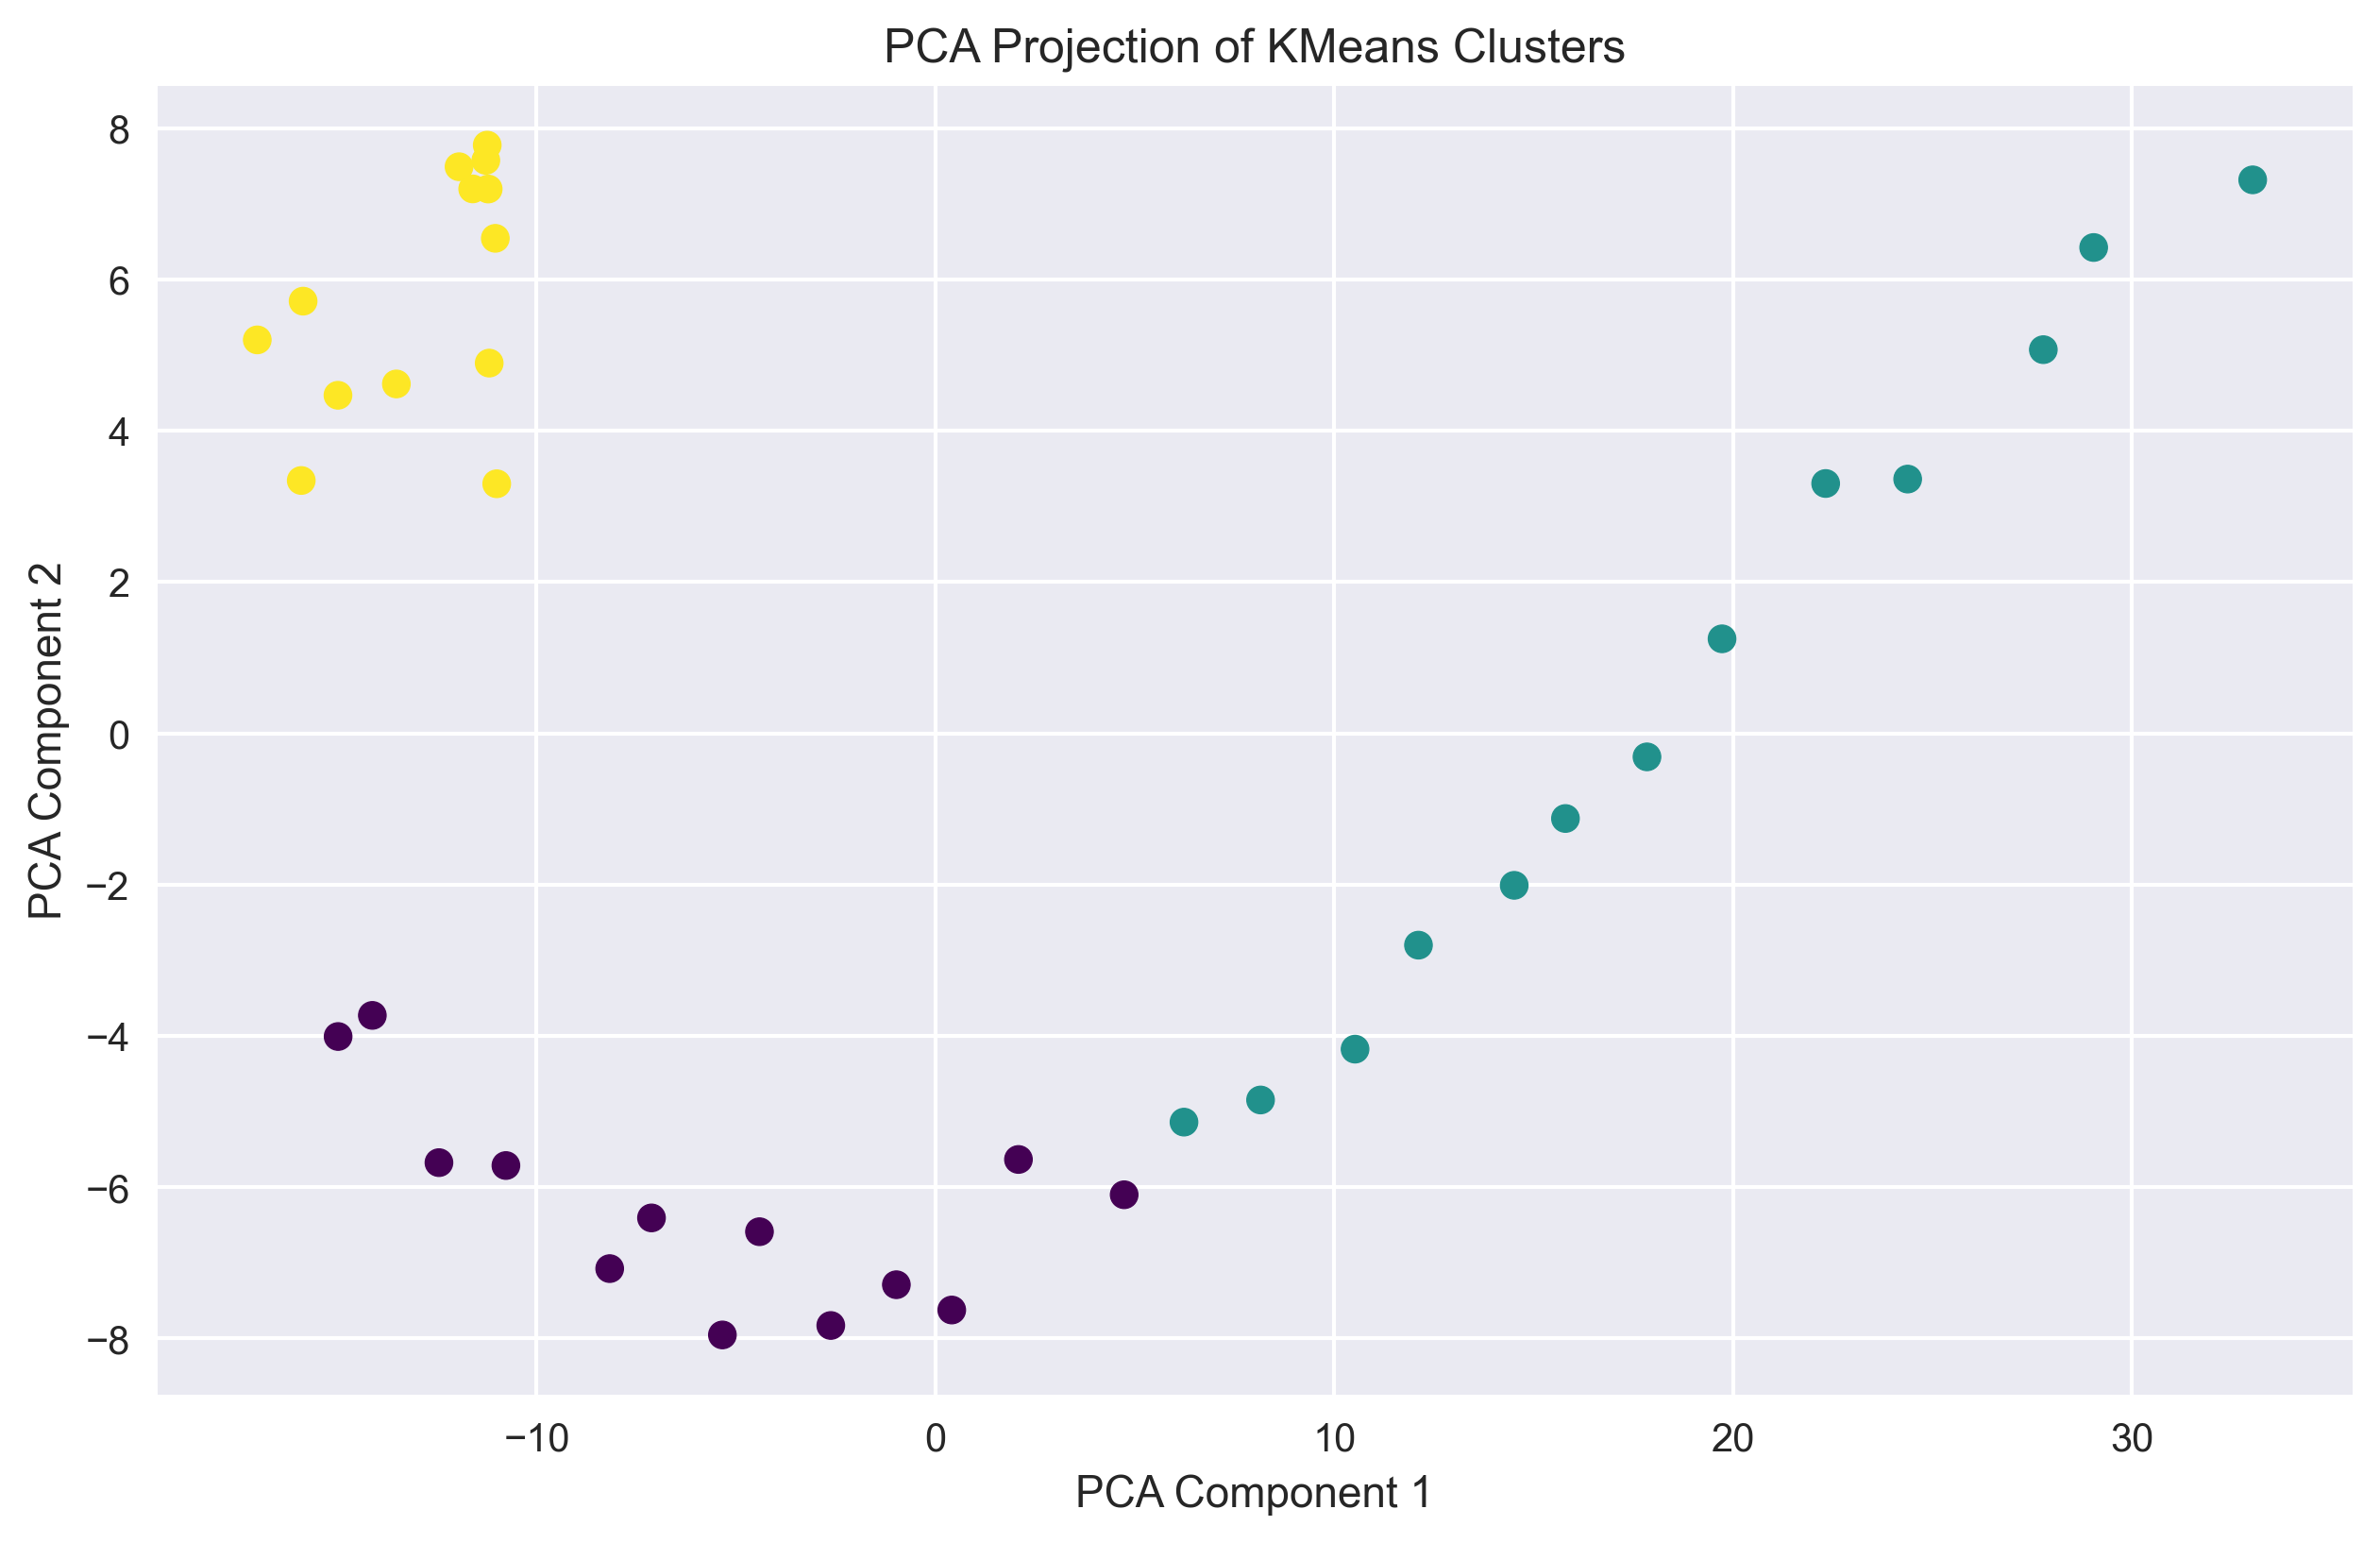
\includegraphics[width=0.8\textwidth]{../clustering.png}
		\caption{PCA projection of KMeans clusters, showing three socioeconomic phases.}
		\label{fig:clustering}
	\end{figure}
	
	\subsection{Performance Improvement}
	Hyperparameter tuning significantly improves Random Forest performance (R²: 0.96 vs. 0.92 for regression; accuracy: 0.88 for classification) \citep{breiman}. MLP improvements are minimal due to dataset size constraints \citep{goodfellow}. The DNN benefits from early stopping, maintaining stable performance across tasks \citep{tensorflow}.
	\section{Discussion and Recommendations}
	This study demonstrates the efficacy of machine learning in analyzing Rwanda's socioeconomic indicators, with Random Forest outperforming other models in regression due to its ability to handle non-linear relationships \citep{breiman}. The DNN and Random Forest excel in classification, capturing complex patterns, while KMeans clustering reveals Rwanda's economic evolution, with the modern growth phase (2011–2024) driven by net ODA, urban population growth, and trade policies \citep{rwanda_vision, eac}. These findings align with Rwanda's Vision 2050 goals and the EAC's development strategy, emphasizing trade and infrastructure as key drivers \citep{un_sdg}.
	
	\subsection{Limitations}
	\begin{itemize}
		\item \textbf{Dataset Size}: The cleaned dataset (39 years) limits neural network performance, favoring tree-based models like Random Forest \citep{goodfellow}.
		\item \textbf{Missing Data}: Dropping indicators with >20\% missing values reduces feature diversity, potentially omitting relevant variables \citep{imputation}.
		\item \textbf{Lack of Text Data}: The dataset excludes qualitative indicators (e.g., policy texts), limiting sentiment or text-based analysis \citep{nlp_book}.
		\item \textbf{Small Test Set}: The classification test set (8 samples) may inflate metrics, reducing generalizability \citep{hastie}.
		\item \textbf{Feature Selection}: Manual selection of indicators may miss latent relationships, addressable via automated methods \citep{feature_selection}.
	\end{itemize}
	
	\subsection{Comparison to Prior Studies}
	Previous studies on EAC economies often rely on econometric models, which assume linear relationships and struggle with complex datasets \citep{eac}. This study's machine learning approach, particularly Random Forest (R²: 0.96) and DNN, outperforms linear models (R²: 0.85), aligning with findings that ensemble and neural methods excel in high-dimensional data \citep{geron, hastie}. Clustering results corroborate historical analyses of Rwanda's development phases, with distinct periods reflecting policy shifts \citep{wdi, rwanda_vision}. Unlike prior work, this study integrates regression, classification, and clustering, providing a holistic view of Rwanda's economic trends \citep{un_sdg}.
	
	\subsection{Recommendations}
	\begin{itemize}
		\item \textbf{Policy}: Strengthen trade facilitation and urban infrastructure to sustain export growth, as indicated by high-export clusters and feature importance \citep{rwanda_vision, eac}.
		\item \textbf{Future Research}: Incorporate multivariate time-series models (e.g., ARIMA, LSTM) to capture temporal dependencies and spatial data from other EAC countries for regional analysis \citep{time_series}.
		\item \textbf{Model Improvement}: Explore ensemble methods combining Random Forest and DNN, and test advanced clustering algorithms like DBSCAN to handle non-spherical clusters \citep{clustering_metrics}.
		\item \textbf{Data Expansion}: Integrate text-based indicators (e.g., policy documents) using natural language processing to enhance predictive models \citep{nlp_book}.
		\item \textbf{EAC Collaboration}: Leverage findings to inform EAC-wide economic strategies, aligning with sustainable development goals \citep{un_sdg}.
	\end{itemize}
	
	\section{References}
	\bibliographystyle{plain}
	\begin{thebibliography}{9}
		\bibitem{wdi}
		World Bank, ``World Development Indicators: Rwanda,'' 2025. Available at: \url{https://api.worldbank.org/v2/en/country/RWA?downloadformat=csv}.
		\bibitem{rwanda_vision}
		Government of Rwanda, ``Vision 2020 and Vision 2050: National Strategy for Transformation,'' 2020. Available at: \url{https://www.minecofin.gov.rw}.
		\bibitem{eac}
		East African Community, ``EAC Development Strategy 2021–2026,'' 2023. Available at: \url{https://www.eac.int}.
		\bibitem{geron}
		Géron, A., ``Hands-On Machine Learning with Scikit-Learn, Keras, and TensorFlow,'' 2nd ed., O'Reilly Media, 2019.
		\bibitem{hastie}
		Hastie, T., Tibshirani, R., and Friedman, J., ``The Elements of Statistical Learning: Data Mining, Inference, and Prediction,'' 2nd ed., Springer, 2009.
		\bibitem{scikit-learn}
		Pedregosa, F., et al., ``Scikit-learn: Machine Learning in Python,'' Journal of Machine Learning Research, vol. 12, pp. 2825–2830, 2011.
		\bibitem{tensorflow}
		Abadi, M., et al., ``TensorFlow: Large-Scale Machine Learning on Heterogeneous Systems,'' 2015. Available at: \url{https://www.tensorflow.org}.
		\bibitem{breiman}
		Breiman, L., ``Random Forests,'' Machine Learning, vol. 45, pp. 5–32, 2001.
		\bibitem{goodfellow}
		Goodfellow, I., Bengio, Y., and Courville, A., ``Deep Learning,'' MIT Press, 2016.
		\bibitem{pandas}
		McKinney, W., ``Data Structures for Statistical Computing in Python,'' Proceedings of the 9th Python in Science Conference, pp. 51–56, 2010.
		\bibitem{matplotlib}
		Hunter, J. D., ``Matplotlib: A 2D Graphics Environment,'' Computing in Science and Engineering, vol. 9, pp. 90–95, 2007.
		\bibitem{seaborn}
		Waskom, M., ``Seaborn: Statistical Data Visualization,'' Journal of Open Source Software, vol. 6, no. 60, 2021.
		\bibitem{imputation}
		Little, R. J. A., and Rubin, D. B., ``Statistical Analysis with Missing Data,'' 3rd ed., Wiley, 2020.
		\bibitem{clustering_metrics}
		Rousseeuw, P. J., ``Silhouettes: A Graphical Aid to the Interpretation and Validation of Cluster Analysis,'' Journal of Computational and Applied Mathematics, vol. 20, pp. 53–65, 1987.
		\bibitem{kingma_adam}
		Kingma, D. P., and Ba, J., ``Adam: A Method for Stochastic Optimization,'' arXiv preprint arXiv:1412.6980, 2014.
		\bibitem{nlp_book}
		Jurafsky, D., and Martin, J. H., ``Speech and Language Processing,'' 3rd ed., Prentice Hall, 2020.
		\bibitem{feature_selection}
		Guyon, I., and Elisseeff, A., ``An Introduction to Variable and Feature Selection,'' Journal of Machine Learning Research, vol. 3, pp. 1157–1182, 2003.
		\bibitem{time_series}
		Hyndman, R. J., and Athanasopoulos, G., ``Forecasting: Principles and Practice,'' 3rd ed., OTexts, 2021.
		\bibitem{un_sdg}
		United Nations, ``Sustainable Development Goals: Agenda 2030,'' 2015. Available at: \url{https://sdgs.un.org}.
	\end{thebibliography}
	
\end{document}